\chapter{Close Coupling $R$-Matrix Theory and Distorted Wave Theory}
\label{chap_bprm_rdw_theory}

\section{Introduction}
The suites of codes that are used in my current work to generate the atomic radiative data, i.e. oscillator strength and photoionization cross section, were developed initially for solving the electron-ion collision problems. One difference between the processes involved in photoionization and electron collision is the projectile, i.e. photons for photoionization and electrons for electron collision. However, they do share the similar final process, i.e. a system consisting of a final target ion and an outgoing electron. Thus these packages used in electron collision problems were extended to calculate the radiative data, for example Opacity Project \citep{opcd_1, opcd_2} and Iron Project \citep{ip_1}. Depending on how the coupling among channels is treated, the methodologies can be separated into two categories, one considers the coupling, i.e. close coupling approximation, and the other neglects such coupling completely, which simplifies into a single-channel problem, i.e. distorted wave approximation. In close coupling approximation, there are several approaches to the electron-ion collision problems, i.e. solving the coupled integro-differential equations, such as IMPACT \citep{impact_3, impact_1, impact_2}, $R$-Matrix \citep{rm_1, rm_2, rm_3}, etc., which solve the same physical problems, only differring by the numerical techniques used in these packages. And a comparision between these two packages can be found in \citet{comp_impact_rm}. In the distorted wave approximation, which is based on the assumption that the coupling between channels is weak, coupled integro-differential equations reduce to a single-channel differential equation, and a good review on different versions of this approximation can be found in \citet{dw_review_1}.

In the following section, solving the coupled integro-differential equations is outlined using close coupling approximation $R$-Matrix approach and distorted wave approximation. As the atomic nuclear charge $Z$ increases, the relativistic effects become more and more important, thus for low-$Z$ elements, non-relativistic treatment is enough, but for medium- and high-$Z$ atoms/ions, relativistic effect has to be included. Therefore, in the above two approximations, non-relativistic and relativistic versions of them are discussed.

\section{Collision Theory -- Solving the Coupled Integro-Differential Equations}
The electron-ion collision problem can be described by the time-independent Schr\"odinger equation
\begin{equation} \label{eq_schodinger}
	H^{N+1}\Psi = E\Psi
\end{equation}
where $E$ is the total energy of the ion + electron system. The Hamiltonian of the system in atomic units is 
\begin{equation} \label{eq_hamiltonian}
	H^{N+1} = \sum_{n=1}^{N=1} (-\frac{1}{2}\nabla_n^2-\frac{Z}{r_n}+\sum_{m>n}^{N+1}\frac{1}{r_{nm}})
\end{equation}
where the first two terms denote the one-electron term, while the last one two-electron term, $r_n$ is the distance between the electron and the nucleus with atomic number $Z$, and $r_{nm} = |\textbf{r}_n-\textbf{r}_m|$ is the  inter-electron distance in which $\textbf{r}_n$ is the vector drawn from the nucleus. The relativistic effects are neglected for the time being. The eigen-wavefunction $\psi_k$ can be expanded in terms of a set of $N$-electron target wavefunctions $\Phi$ and the wavefunction of the colliding electron $\theta$
\begin{align}
	\psi_k(x_1\cdot\cdot\cdot x_{N+1}) &= \mathcal{A}\sum_{i}\Phi_i(x_1\cdot\cdot\cdot x_{N})\theta_i(x_{N+1}) \label{wave_expand}\\
	\theta_i(x) &=Y_{li}^{m_{li}}(r)\delta(m_{si}|\sigma)\frac{1}{r}F_i(r)
\end{align}
where $k$ characterizes the initial conditions and usually denotes the collision channel, $\mathcal{A}$ is antisymmetrization operator, $x_n$ denotes the space and spin coordinates of the nth electron, $Y_l^m$ is a sphyerical harmonic, $\sigma$ is a spin coordinate, $F_i(r)$ describes the radial part of the colliding electron. The target state $\Phi_i$ can be written as a configuration interaction expansion in terms of some basis configurations $\phi_i$ by
\begin{equation} \label{eq_target_expand}
	\Phi_i(x_1\cdots x_N) = \sum_kb_{ik}\phi_k(x_1\cdots x_N)
\end{equation}
where the configuration mixing coefficients $b_{ik}$ are determined by diagonalizing the target Hamiltonian in the basis of $\phi_k$. The target Hamiltonian is defined by equation \ref{eq_hamiltonian} with $N+1$ replaced by $N$ and the energy of state $\Phi_i$ is defined by
\begin{equation} \label{eq_dia_target}
	\langle\Phi_i|H^N|\Phi_j\rangle=E_i^N\delta_{ij}
\end{equation}
The configurations $\phi_i$ are constructed from a bound orbital basis consisting of self consistent field orbitals plus some additional pseudo-orbitals included to model electron correlation effect. The expansion of $\Phi_i$ in the basis of $\phi_k$ is just like the Slater determinant, which treats fully the antisymmetric requirement of the wavefunctions for a system of fermions. The radial parts of these one-electron orbitals, $P_{nl}(r)$, satisfy the orthonormality conditions 
\begin{equation}
	\langle P_{n_il}|P_{n_jl} \rangle = \int_{0}^{\infty} P_{n_il}(r)P_{n_jl}(r)dr=\delta_{n_in_j}
\end{equation}
The radial functions $P_{nl}(r)$ are provided externally from other atomic structure packages, e.g. SUPERSTRUCTURE \citep{ss_1, ss_2, ss_3}, and a brief description of SUPERSTRUCTURE can be found in Appendix \ref{app_bprm_code}. 

Pincipally the target states $\Phi_i$ included in the expansion are complete, however, in practice they are included partly with the ones of interest. And expansion \ref{wave_expand} can be rewritten in the following form
\begin{multline} \label{eq_full_expand}
	\psi_k(x_1\cdot\cdot\cdot x_{N+1}) = \mathcal{A}\sum_{i}^{n}\overline{\Phi}_i(x_1\cdot\cdot\cdot x_{N}; \hat{\textbf{r}}_{N+1}\sigma_{N+1}) \frac{1}{r_{N+1}} F_{ik}(r_{N+1}) \\+ \sum_{j=1}^m d_{jk} \chi_j(x_1\cdots x_{N+1}) 
\end{multline}
where $n$ is the number of channels; $\overline{\Phi}_i$ is the channel function, which is obtained by coupling the target state $\Phi_i$ with the angular and spin functions of the colliding electron to form the total angular momentum and parity, $F_{ik}$ is the radial component of the colliding electron wavefunction and called channel orbitals, and $\chi_j$ is the $(N+1)$-electron bound state function, which is formed by the one-electron atomic wavefunctions. To allow for fast convergence numerically, an orthogonality condition is usually required for $l_i = l_j$
\begin{equation} \label{eq_bound_free_orth}
	\langle P_{n_jl_j}|F_{ik}\rangle = \int_{0}^{\infty}P_{n_jl_j}(r)F_{ik}(r)dr=0
\end{equation}
, in which case the second term in equation \ref{eq_full_expand} has to be introduced, serving two purposes. Part of the states included in the second term are to ensure the completeness of the expansion of the target-electron wavefunctions. In the electron-ion collision problem, the colliding electron can be free after collision, or can be captured by the target. The orthogonality condition of equation \ref{eq_bound_free_orth} means the radial wavefunction of the colliding electron projects out of the subshell space of the target, which can be interpreted as keeping the colliding electron from being captured into any incomplete subshells, and this phenomenon is described in the first term of the expansion \ref{eq_full_expand}. It represents a free channel expansion, because the channel orbitals $F_{ik}$ can be freely varied. To be complete, the fact that the colliding electron can be captured by the target needs to be addressed, which is exactly what the second term in expansion \ref{eq_full_expand} describes, i.e. an $(N+1)$-electron system with one-electron atomic wavefunctions for all electrons and these states are constructed using the same target radial functions $P_{nl}$. And this term is called correlation functions, representing the bound channel expansion. And the other states included in the second term of equation \ref{eq_full_expand} is to allow for improved description of short-range electron correlation effects. To elaborate on how to choose the $(N+1)$-electron bound channel configurations, for example, if $Ck_jl_j$ represents a free channel term, where $C$ denotes the target state configuration, then after imposing the orthogonality condition, it is necessary to include in the second term a bound channel configuration $Cnl$. More examples can be found in \citet{dw_review_1, henry_1993}. To solve for the channel orbitals $F_i(r)$, we can substitute wavefunction \ref{eq_full_expand} into Sch\"odinger equation \ref{eq_schodinger}, project onto the channel functions $\overline\Phi_i$ and functions $\chi_j$, separte out the spin and angular variables and eliminate the coefficients $d_{jk}$, and finally obtain the following set of coupled integro-differential equations \citep{bspline_2006}
\begin{equation} \label{eq_coupled_intdiff}
	\Bigg(\frac{d^2}{dr^2} - \frac{l_i(l_i+1)}{r^2} + \frac{2Z}{r} + k_i^2\Bigg) F_i(r) = 2 \sum_j(V_{ij}+W_{ij}+X_{ij})F_j(r)
\end{equation}
where $l_i$ is the orbital angular momentum of the colliding electron, $V_{ij},~W_{ij}$ and $X_{ij}$ are the partial-wave decompositions of the local direct, non-local exchange and non-local correlation potentials, whch generally are too complicated to write down explicitely. This equation is the core of electron-ion collision theory, and close coupling approximation considers such coupling and exchange terms, while distored wave approximation neglects them. In the following section, these two approximations are outlined.

\subsection{$R$-Matrix Approach}
To solve the coupled integro-differential equation \ref{eq_coupled_intdiff}, \citet{rm_1} developed the $R$-Matrix approach, which starts by dividing the configuration sapce into two regions, i.e. internal region and external region. See figure \ref{figure_rm_space}. When the colliding electron interacts with the target ion, in the internal region, the electron is indistinguishable from the other electrons belonging to the target ion, while in the external region, it is far away from these target electrons and explicitly distinguishable. Thus, in the internal region, instead of solving the coupled integro-differential equations, we can treat the $(N+1)$-electron wavefunction as an expansion of an energy-independent basis set, just like the $N$-electron target, including the exchange and other correlation effects. In the external region, electron exchange and correlation effects between the target and the colliding electron can be neglected if the $R$-Matrix boundary is chosen large enough that the charge distribution of the target is contained within the sphere, and this can be guaranteed by the radial part of the target wavefunciton being negligibly samll. However, the channel orbitals $F_i(r=a)$ should be non-zero, which provides a link between the solution in the internal and external regions.

%======= FIGURE: 
\begin{figure}
	\centering
	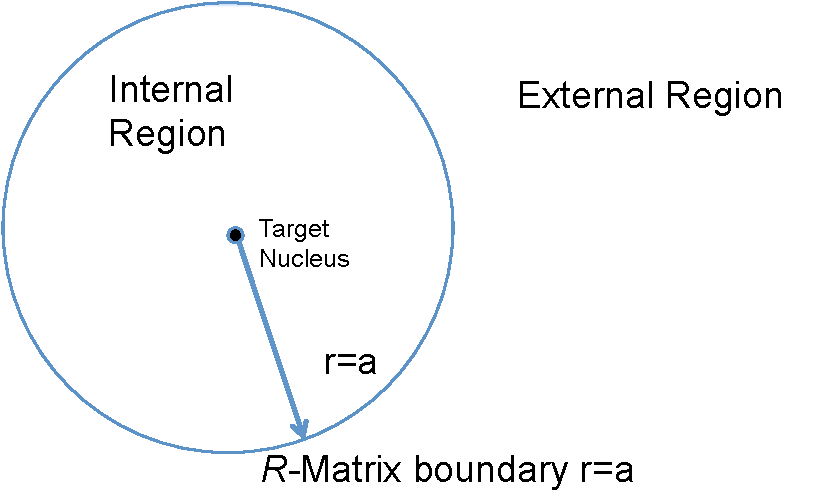
\includegraphics[width=.9\textwidth]{figures_3/r_matrix_box}	
	\caption{The partition of the configuration space in $R$-Matrix approach.}
	\label{figure_rm_space}
\end{figure}

In section \ref{sec_nr_rm}, the procedure of solving for the channel orbitals in internal and external regions will be outlined, which closely follows \citet{rm_3}, and this is the non-relativistic version of $R$-Matrix approach. In section \ref{sec_r_rm}, the relativistic effects \citep{rm_2} are included in the Hamiltonian and the difference from the non-relativistic version is discussed.

\subsubsection{Non-Relativistic} \label{sec_nr_rm}
In the internal region, the target wavefunctions are expanded as in equation \ref{eq_target_expand}, but the basis of the channel orbitals needs to be determined. Practically the basis $u_{ij}(r)$ satisfying the following single-channel scattering equation is adopted
\begin{equation} \label{eq_single_channel}
	\Bigg(\frac{d^2}{dr^2} - \frac{l_i(l_i+1)}{r^2} + V_0(r) + k_{ij}^2\Bigg) u_{ij}(r) = \sum_{n=1}^{NRANG2} \Lambda_{ijn} P_{nl_i}(r)
\end{equation}
with the boundary conditions
\begin{equation} \label{eq_boundary_condition}
	\begin{split}
		u_{ij}(0) &= 0 \\
		\Bigg(\frac{a}{u_{ij}(a)} \Bigg) \Bigg(\frac{du_{ij}}{dr} \Bigg)_{r=a} &=b
	\end{split}
\end{equation}
where $NRANG2$ is the number of continuum basis included in the calculation; the Lagrange multipliers $\Lambda_{ijn}$ ensure the continuum basis orthogonal to the bound orbitals $P_{nl_i}(r)$ of the same angular symmetry; the potential $V_0(r)$ behaves like $\frac{2Z}{r}$, which is not crucial; $k_{ij}^2$ is the energy of the colliding electron in $Ry$; b is arbitrary, and is normally set to 0. An algorithm about generating such basis can be found in \citet{cont_orbital}.

The continuum basis $u_{ij}(r)$ is orthogonal to both themselves and the bound orbitals within the $R$-Matrix boundary $r=a$
\begin{equation}
	\begin{split}
		(u_{ij}|u_{ij'}) &= 0\\
		(u_{ij}|P_{nl_i}) &= 0
	\end{split}
\end{equation}
where the round brackets indicate the integration range is from 0 to a. Since the bound orbitals $P_{nl_i)}(r)$ is orthoganal to the channel orbital $F_i(r)$ in the whole range and $P_{nl_i}(r>a)$ is negligibly small, thus it is equivalent to $(u_{ij}|P_{nl_i}) = 0$.

Therefore for each channel i, a complete set of basis is formed within $R$-Matrix boudary
\begin{equation}
	P_{n_{min}l_i}, \cdots, P_{n_{max}l_i}, u_{i1}, u_{i2}, \cdots, u_{i NRANG2}
\end{equation}
where $n_{min} = l_i+1$, and the total eigen-wavefunction $\psi_k$ can be expanded in such basis, independent of the total energy $E$. Thus equation \ref{eq_full_expand} can be rewritten as
\begin{multline} \label{eq_full_expand_cont_basis}
	\psi_k(x_1\cdot\cdot\cdot x_{N+1}) = \mathcal{A}\sum_{i=1}^{n}\sum_{j=1}^{NRANG2}c_{ijk}\overline{\Phi}_i(x_1\cdot\cdot\cdot x_{N}; \hat{\textbf{r}}_{N+1}\sigma_{N+1}) \frac{1}{r_{N+1}} u_{ij}(r_{N+1}) \\+ \sum_{j=1}^m d_{jk} \chi_j(x_1\cdots x_{N+1}) 
\end{multline}
where $c_{ijk}$ and $d_{ik}$ can be determined by diagonalizing 
\begin{equation} \label{eq_diag_np1}
	(\psi_k|H^{N+1}|\psi_{k'}) = E_k\delta_{kk'}
\end{equation}

The total wavefunction of $(N+1)$-electron system within $R$-Matrix boundary can be expanded as 
\begin{equation}
	\Psi = \sum_k A_{EK} \psi_k
\end{equation}
where $A_{EK}$ is the coefficient that is energy independent. Define
\begin{equation}
	\frac{1}{r}w_{ik}(r) = \sum_j c_{ijk}u_{ij}(r) = (\overline{\Phi}_i|\psi_k)
\end{equation}
and the reduced radial wavefunction of the colliding electron
\begin{equation}
	\frac{1}{r}F_i(r) = \frac{1}{r} \sum_k A_{EK} w_{ik}(r) = (\overline{\Phi}_i|\Psi)
\end{equation}
It can be shown that $A_{EK}$ can be written as the following form
\begin{equation}
	A_{EK} = \frac{1}{2a} (E_k-E)^{-1} \sum_i w_{ik}(a) \Bigg( a\frac{dF_i}{dr} - bF_i \Bigg)_{r=a}
\end{equation}

\begin{equation} \label{eq_rm_a}
	F_i(a) = \sum_j R_{ij}(E) \Bigg( a\frac{dF_j}{dr} - bF_j \Bigg)_{r=a}
\end{equation}
where $R$-Matrix is defined as 
\begin{equation} \label{eq_rm_boundary}
	R_{ij}(E) = \frac{1}{2a} \sum_k \frac{w_{ik}(a)w_{jk}(a)}{E_k - E}
\end{equation}
The surface amplitude $w_{ik}(a)$ and poles $E_k$ are obtained directly from the eigenvectors and eigenvalues of the Hamiltonian matrix defined in equation \ref{eq_diag_np1}. And $R$-matrix is obtained for all energies by diagonalizing $H^{N+1}$ once for each symmetry, and this is the advantage of $R$-Matrix method when computing at numerious energies, especially in the resonance region. The reduced radial wavefunction $F_i(a)$ is to be matched with the solution in the external region.

As the summation in equation \ref{eq_rm_boundary} is truncated to some finite number of terms, the other distant, neglected terms can play an important role in the diagonal elements of the $R$-matrix where they add coherently. These neglected terms can be included by solving the differential equation
\begin{equation}
\Bigg(\frac{d^2}{dr^2} - \frac{l_i(l_i+1)}{r^2} + V_0(r) + k_{i}^2\Bigg) u_{i}^0(r) = \sum_{k} \Lambda_{ijk} P_k(r)
\end{equation}
, which is the same as equation \ref{eq_single_channel}, but is solved at channel energies $k_i^2$ without applying the boundary condition equations \ref{eq_boundary_condition} at $r=a$. Suppose the $R$-Matrix is calculated from the first $N$ terms in the continuum expansion, the correction to the diagonal elements of the $R$-Matrix at the energy $k_i^2$ is 
\begin{equation}
	\begin{split}
		R_{ii}^c (N, k_i^2) &\approx \frac{1}{a} \sum_{j=N+1}^{\infty} \frac{u_{ij}(a)^2}{k_{ij}^2-k_i^2} \\
		& = \Bigg[ \frac{a}{u_i^0(a)} \Bigg( \frac{du_i^0}{dr} \Bigg)_{r=a} -b \Bigg]^{-1} - \frac{1}{a} \sum_{j=1}^{N} \frac{u_{ji}(a)^2}{k_{ij}^2 - k_i^2}
	\end{split}
\end{equation}
, where $u_{ij}(r)$ refers to the jth eigensolution of equation \ref{eq_single_channel} with the boundary condition, and $u_i^0$ is the solution without boundary condition. We therefore use the corrected $R$-Matrix in place of equation \ref{eq_rm_boundary}
\begin{equation}
R_{ij}(E) = \frac{1}{2a} \sum_k \frac{w_{ik}(a)w_{jk}(a)}{E_k - E} +R_{ii}^c(N, k_i^2)\delta_{ij}
\end{equation}

At this point the theoretical methods applied in the internal region is described, and we are to solve the integro-differential equations \ref{eq_coupled_intdiff} in the external region, in which the exchange and correlation terms can be neglected, thus the total wavefunction can be written as 
\begin{equation} \label{eq_new_expand}
	\Psi(x_1\cdot\cdot\cdot x_{N+1}) = \sum_{i}^{n}\overline{\Phi}_i(x_1\cdot\cdot\cdot x_{N}; \hat{\textbf{r}}_{N+1}\sigma_{N+1}) \frac{1}{r_{N+1}} F_{i}(r_{N+1}) 
\end{equation}
where $\overline{\Phi}_i$ are the same as those used in the internal region, but with no exchange between the target electrons and the colliding electron. After substituting equation \ref{eq_new_expand} into Schr\"odinger equation and projecting onto the channel functions, we obtain the following coupled differential equations
\begin{equation}
\Bigg(\frac{d^2}{dr^2} - \frac{l_i(l_i+1)}{r^2} +\frac{2Z}{r} + k_{i}^2\Bigg) F_{i}(r) = 2\sum_{j=1}^n V_{ij} F_j(r)
\end{equation}
, which can be reduced to
\begin{equation}\label{eq_ex_diff}
	\Bigg(\frac{d^2}{dr^2} - \frac{l_i(l_i+1)}{r^2} +\frac{2(Z-N)}{r} + k_{i}^2\Bigg) F_{i}(r) = 2\sum_{\lambda=1}^{\lambda_{max}} \sum_{j=1}^{n} \frac{a_{ij}^\lambda}{r^{\lambda+1}} F_j(r) 
\end{equation}
, where $n$ is the number of channels in the expansion, $l_i$ and $k_i^2$ are the channel angular momenta and energies, $N$ is the number of electron in the target, $a_{ij}^\lambda$ is the long-range potential coefficients. In BPRM code (see Appendix \ref{app_bprm_code}), such long-range multipole potentials on the right hand side of equation \ref{eq_ex_diff} is treated with two options. One is to neglect (IPERT = 0) them, and the other is to treat them as a perturbation (IPERT = 1) with $\lambda = 1,~2$ \citep{opcd_2}.

The asymptotic form of the channel orbitals $F_i(r)$ at infinity is
\begin{equation} \label{eq_f_asymptotic}
	F_{ij}(r) \underset{r \to \infty}{\sim}
	\begin{cases}
		k_i^{-1/2}(sin\theta_i\delta_{ij}+cos\theta_iK_{ij}), & \text{open~channels} \\
		exp(-\phi_i)\delta_{ij}, & \text{close~channels}
	\end{cases}
\end{equation}
, where the second index $j$ on $F_{ij}$ denotes the linearly independent solutions of equation \ref{eq_ex_diff}, and 
\begin{align}
	\theta_i &= k_ir-\frac{1}{2}l_i\pi-\eta_iln2k_ir+arg\Gamma (l_i+1+i\eta _i) \label{eq_theta}\\
	\eta_i &= -\frac{z}{k_i} \\
	\phi_i &= |k_i|r - \frac{z}{|k_i|}ln (2|k_i|r) \label{eq_phi}
\end{align}
, where $z=Z-N$ is the residual target charge.

In principle, we can integrate equation \ref{eq_ex_diff} outwards subject to the $R$-matrix boundary condition of equations \ref{eq_rm_a}, and fit to the asymptotic form of equation \ref{eq_f_asymptotic}, however, the open channel solution is not fully determined until the reactance matrix $K$ in equation \ref{eq_f_asymptotic} is found.

When calculating the radiative data, i.e. oscillator strength and photoioization cross section, we need the wavefunctions of bound states (all channels are closed) and free states (at least one channel is open), thus at this point where we have discussed the techniques used in the internal and external regions, we are ready to link the solutions in these two regions.

To find the solution for the bound states, we can define $n$ linearly  independent solutions of the external region equation \ref{eq_ex_diff}, which satisfy the following boundary condition
\begin{equation}
	c_{ij}(r) \underset{r \to \infty}{\sim} exp(-\phi_i)\delta_{ij} \qquad i = 1,n \quad j = 1, n
\end{equation}
, where $\phi_i$ is given by \ref{eq_phi}. We can expand external solution in terms of those solutions
\begin{equation}
	F_i(r) = \textbf{cx} = \sum_{j=1}^n c_{ij}(r)x_j \qquad i = 1,n 
\end{equation} 
, where $x_j$ can be determined by substituting this expression for $F_i$ into the interal wavefunction at the boundary $r=a$
\begin{equation} \label{eq_frmb}
	\mathbf{F} = a\textbf{R} \cdot \dot{\mathbf{F}} - b \mathbf{R} \cdot \mathbf{F}
\end{equation}
, where $\dot{\mathbf{F}} = d\mathbf{F}/dr$. We get the following $n$ homogeneous equations 
\begin{equation}
	\mathbf{cx} = a \mathbf{R\dot{c}x} - b \mathbf{Rcx}
\end{equation}
Solving for $\mathbf{x}$ with nontrivial solutions, we find the condition is 
\begin{equation}
	\text{det}~ \mathbf{B} = 0
\end{equation}
, where $\mathbf{B} = \mathbf{c} - a \mathbf{R}(\dot{\mathbf{c}}- \frac{b}{a}\mathbf{c})$, thus the wavefunctions and energy levels for the bound states are solved.

To find the solutions for the free states, a similar method as for the bound states can be adopted. In this case, we introduce $(n+n_a)$ linearly independent solutions $s_{ij}(r)$ and $c_{ij}(r)$ of equation \ref{eq_ex_diff}, satisfying the following boundary conditions
\begin{equation}
	\begin{rcases}
		s_{ij}(r) \\
		c_{ij}(r) \\
		c_{ij}(r) \\
	\end{rcases}
	\underset{r \to \infty}{\sim} 
	\begin{cases}
	sin\theta_i\delta_{ij} 	& i=1,n \qquad j = 1,n_a\\
	cos\theta_i\delta_{i, j-n_a} & i=1,n \qquad j = 1,n_a\\
	exp(-\phi_i)\delta_{i,j-n_a} & i=1,n \qquad j = n_a+1,n \\
	\end{cases}
\end{equation}
, where $\theta_i$ and $\phi_i$ are defined as \ref{eq_theta} and \ref{eq_phi}, respectively. Thus the reduced radial wavefunction $F_{ij}(r)$ can be expanded as
\begin{equation}
	\mathbf{F=s+cK}
\end{equation}
After substituting it into equation \ref{eq_frmb} and solving for $\mathbf{K}$, we have
\begin{equation}
	\mathbf{K=B^{-1}A}
\end{equation}
, where $\mathbf{A} = -\mathbf{s} +a\mathbf{R}(\dot{\mathbf{s}}-\frac{b}{a}\mathbf{s})$, $\mathbf{B} = \mathbf{c} +a\mathbf{R}(\dot{\mathbf{c}}-\frac{b}{a}\mathbf{c})$. Thus the entire wavefunctions of the free states are solved.


\subsubsection{Relativistic} \label{sec_r_rm}
For medium heavy element like iron, the relativistic effects should be included and the Breit-Pauli Hamiltonian is sufficient, which results from the reduction of the Dirac equation and Breit interaction to Pauli form \citep{rm_2, scott_bprm}. The Breit-Pauli Hamiltonian can be written as
\begin{equation}
	H_{BP}^{N+1} = H_{NR}^{N+1} + H_{REL}^{N+1} 
\end{equation}
, where $H_{NR}^{N+1}$ is defined as equation \ref{eq_hamiltonian}, and $H_{REL}^{N+1}$ consists of the one-body operators that are given by 
\begin{subequations}
	\begin{align}
		H_{mass}^{N+1} &= -\frac{1}{8}\alpha^2 \sum_{i=1}^{N+1} \nabla_i^4 \qquad \text{the mass-correction term}\\
		H_D^{N+1} &= -\frac{1}{8}\alpha^2 Z \sum_{i=1}^{N+1} \nabla_i^4 (\frac{1}{r_i}) \qquad \text{the one-body Darwin term}\\
		H_{SO}^{N+1} &= \frac{1}{2}\alpha^2 Z \sum_{i=1}^{N+1} \frac{1}{r_i^3} (\mathbf{l}_i\cdot \mathbf{S}_i) \qquad \text{the spin-orbit interaction}
	\end{align}
\end{subequations}
$H_{NR}^{N+1},~H_{mass}^{N+1} and H_D^{N+1}$ commute with $\mathbf{L}^2$, $\mathbf{S}^2$, $\mathbf{L}_Z$,  $\mathbf{S}_Z$ and parity, while $H_{BP}^{N+1}$ only commutes with $\mathbf{J}^2$, $\mathbf{J}_Z$ and parity.

This difference in the Hamiltonian from the non-relativistic version of $R$-Matrix theory affects several aspects of the Breit-Pauli $R$-Matrix theory. One is in the diagonalization of equations \ref{eq_dia_target} and \ref{eq_diag_np1} , where the Breit-Pauli Hamiltonian is used. And the angular coupling scheme is changed to $jK$ pair coupling
\begin{equation}
	\mathbf{J}_i +\mathbf{l} = \mathbf{K} \qquad \mathbf{K+\frac{1}{2}=J}
\end{equation}
, where $J_i$ is the total angular momentum of the target state. And this results in a much larger Hamiltonian matrix, which requires considerably more computational effort. The rest of the method is the same as the non-relativistic version.



\subsection{Distorted Wave Approximation}
In this section, a much simpler approximation than the close coupling is discussed. We will briefly introduce the non-relativistic distorted wave approximation, followed by a more detailed fully relativistic distorted wave approximation, which is mainly about the techniques used in flexible atomic code (FAC) \citep{gu_2008}.
\subsubsection{Non-Relativistic}
In the distorted wave approximation, the coupling, exchange and correlation potentials on the right hand side of the integro-differential equation \ref{eq_coupled_intdiff} are neglected. Thus with the non-relativistic Hamiltonian, it reduces to a single-channel differential equation \citep{book_int_diff}
\begin{equation}
\Bigg(\frac{d^2}{dr^2} - \frac{l_i(l_i+1)}{r^2} +V_i(r) + k_{i}^2\Bigg) f_{i}(r) = 0
\end{equation}                    
, where $V_i(r)\underset{r \to \infty}{\sim} \frac{2(Z-N)}{r}$. And the boundary condition for $f_i(r)$ is
\begin{subequations}
	\begin{align}
		f_i(0) &= 0 \\
		f_i(r) &\underset{r \to \infty}{\sim} k_i^{-1/2}sin\Bigg( k_ir+\frac{z}{k_i}lnr+\tau_i \Bigg)
	\end{align}
\end{subequations}
With the solutions $f_i(r)$, we construct functions
\begin{equation}
	F_i = f_i - \sum_{\alpha}\delta(l_i, l_\alpha)(f_i|P_\alpha)P_\alpha
\end{equation}
, which satisfy the orthogonality conditions
\begin{equation}
	(F_i|P_\alpha) = 0 \qquad  \text{if} \quad l_i= l_\alpha
\end{equation}
Since the channel coupling is neglected, the radial functions with the boundary condition $i'$ are 
\begin{equation}
	F_{ii'} = F_i \delta_{ii'}
\end{equation}
Thus the coupled expansion \ref{eq_full_expand} can be rewritten as
\begin{multline} \label{eq_full_expand_dw}
	\psi_i(x_1\cdot\cdot\cdot x_{N+1}) = \mathcal{A}\overline{\Phi}_i(x_1\cdot\cdot\cdot x_{N}; \hat{\textbf{r}}_{N+1}\sigma_{N+1}) \frac{1}{r_{N+1}} F_{i}(r_{N+1}) \\+ \sum_{j=1}^m d_{j} \chi_j(x_1\cdots x_{N+1}) 
\end{multline}
Since the current calculation does not use the non-relativistic distorted wave approximation, we will not spend more effort on this topic, more information can be found in \citet{ucl_dw}.


\subsubsection{Relativistic}
The fully relativistic distorted wave code we use is FAC (flexible atomic code), which is developed by Ming Feng Gu \citep{gu_2008}, who applied many of the techniques that were used in the existing code at that time \citep{dw_guoxin, dw_sampson, dw_zhang, hullac}, wrote the code from scratch and made the package available to public. FAC treats the bound and continuum processes altogether, and is very efficient in computing various atomic quantities. In the rest of the section, the methods used for solving for the bound and continuum wavefunctions are described.

The many-electron Dirac Hamiltonian is 
\begin{equation}
	H = \sum_{i=1}^N H_D(i) +\sum_{i<j}^N \frac{1}{r_{ij}}
\end{equation}
, where $N$ is the number of electrons in the atomic system, $H_D(i)$ is the single-electron Dirac Hamiltonian for the potential due to the nuclear charge. The wavefunction of the system can be expanded as
\begin{equation}
	\psi = \sum_\nu b_\nu \Phi_\nu
\end{equation}
, where $b_\nu$ is the coefficients by diagonalizing the total Hamiltonian, $\Phi_\nu$ are the configuration state functions, which are antisymmetric sums of the products of $N$ one-electron Dirac spinors $\varphi_{n\kappa m}$
\begin{equation}
	\varphi_{n\kappa m} = \frac{1}{r}
	\begin{pmatrix}
		P_{n\kappa} (r) \chi_{\kappa m}(\theta, \phi, \sigma) \\
		iQ_{n\kappa} (r) \chi_{-\kappa m}(\theta, \phi, \sigma)
	\end{pmatrix}
\end{equation}
, where $P_{n\kappa}$ and $Q_{n\kappa}$ are the large and small components of the radial function; $\chi_{\kappa m}$ is the usual spin-angular function; $n$ is the principle quantum number; $\kappa$ is the relativistic angular quantum number, which is related to the orbital and total angular momentum by
\begin{equation}
	\kappa = (l-j)(2j+1)
\end{equation}
and $m$ is the $z$-component of the total angular momentum $j$. 

For bound states, the one-electron large and small components,  $P_{n\kappa}$ and $Q_{n\kappa}$, satisfy the following coupled Dirac equations
\begin{equation} \label{eq_dirac_eq}
	\begin{split}
		\Bigg( \frac{d}{dr} + \frac{\kappa}{r} \Bigg) P_{n\kappa} &= \alpha \Bigg( \varepsilon_{n\kappa} - V + \frac{2}{\alpha ^2} \Bigg) Q_{n\kappa} \\
		\Bigg( \frac{d}{dr} - \frac{\kappa}{r} \Bigg) Q_{n\kappa} &= \alpha \Bigg( - \varepsilon_{n\kappa} + V \Bigg) P_{n\kappa}
	\end{split}
\end{equation}
, where $\alpha$ is fine structure constant in atomic unit, and $\varepsilon_{n\kappa}$ are the energy eigenvalues of the raidal functions. The local central potential $V$ includes the contribution from the nuclear charge $V^N(r)$ and the electron-electron interaction $V^{ee}(r)$. The nuclear potential is 
\begin{equation}
	V^N = 
	\begin{cases}
		\frac{Z}{2}\Big(\frac{4}{R_N}\Big)\Big[3-\Big(\frac{r}{R_N}\Big)^2\Big], \qquad & r \leq R_N \\
		Z, & r > R_N
	\end{cases}
\end{equation}
, where $R_N$ is the statistical model radius of the nucleus, which can be expressed in terms of the atomic number $A$, $R_N = 2.2677\times10^{-15}A^{1/3}$. The electron-electron interaction excluding the self-interaction term is 
\begin{multline}
	V^{ee}(r) = \frac{1}{r\sum_a\omega _a\rho _a(r)} \Bigg\{ \sum_{ab} \omega_a(\omega_{ab}-\delta_{ab})Y_{bb}^0(r) \rho_a(r) \\+ \sum_a \omega_a(\omega_a-1)\sum_{k>0} f_k(a, a) Y_{aa}^k(r)\rho_a(r) + \sum_{a \neq b} \sum_k \omega_a \omega_b g_k(a, b)Y_{ab}^k(r) \rho_{ab}(r) \Bigg\}
\end{multline}
, where $a=n\kappa$ and $b=n'\kappa'$ denote the subshells; $\omega_a$ and $\omega_b$ the occupation number of subshells $a$ and $b$, which are usually called mean configuration and about half an electron is excited, and 
\begin{equation}
	\begin{split}
		\rho_{ab} = P_a(r) P_b(r) + Q_a(r) Q_b(r) \\
		Y_{ab}^k(r) = r \int \frac{r_<^k}{r_>^{k+1}} \rho_{ab} (r') dr'
	\end{split}
\end{equation}
, where $r_<$ and $r_>$ are the lesser and greater of $r$ and $r'$, respectively. $f_k$ and $g_k$ are the direct and exchange coefficients defined as 
\begin{equation}
	\begin{split}
		f_k(a, b) &= -
						\Bigg( 1+\frac{1}{2j_a} \Bigg)
						\binom{~~j_a \qquad k \qquad j_b}{-\frac{1}{2} \qquad 0 \qquad \frac{1}{2}} ^2  \\
		g_k(a, b) &= - \binom{~~j_a \qquad k \qquad j_b}{-\frac{1}{2} \qquad 0 \qquad \frac{1}{2}}^2
	\end{split}
\end{equation}
The orthonomality condition satisfied by the bound radial functions is 
\begin{equation} \label{eq_bound_orth}
	\int_0^\infty dr [P_{n\kappa}(r)P_{n'\kappa}(r) + Q_{n\kappa}(r)Q_{n'\kappa}(r)] = \delta_{nn'}
\end{equation}
To solve the coupled Dirac equations \ref{eq_dirac_eq}, we can eliminate the small component and define the following variables
\begin{equation}
	\begin{split}
		P_a &= \xi_a(r) F_a(r) \\
		\xi_a(r) &= \sqrt{1+\frac{\alpha^2}{2}[\varepsilon_a-V(r)]} \\
		Q_a &= \frac{\alpha}{2\xi_a^2} \Bigg( \frac{d}{dr} P_a + \frac{\kappa}{r} P_a \Bigg)
	\end{split}
\end{equation}
, and we have the following equation
\begin{equation} \label{eq_rdw_f}
	\frac{d^2}{dr^2}F_a(r) + \Bigg\{ 2[\varepsilon_a - U(r)] - \frac{\kappa (\kappa+1)}{r^2} \Bigg\}F_a(r) =0
\end{equation}
, where 
\begin{equation}
	\begin{split}
		U(r) &= V(r) - \frac{\alpha^2}{2} \Bigg \{ [V(r)-\varepsilon_a]^2 - W(r) \Bigg\} \\
		W(r) &= \frac{1}{4\xi^2(r)} \Bigg [ \frac{d^2}{dr^2}V(r) + \frac{3\alpha^2}{4\xi^2(r)}\Bigg( \frac{d}{dr} V(r)\Bigg)^2 - \frac{2\kappa}{r} \frac{d}{dr} V(r)\Bigg]
	\end{split}
\end{equation}
After a further transformation with
\begin{equation}
	\begin{split}
		t = t(r) \\
		F_a(r) = \Bigg( \frac{dt}{dr} \Bigg)^{-1/2}G_a(t)
	\end{split}
\end{equation}
, equation \ref{eq_rdw_f} can be transformed into
\begin{multline} \label{eq_rdw_f_final}
	\frac{d^2}{dt^2}G_a(t) = \Bigg( \frac{dt}{dr}\Bigg)^{-2} G_a(t) \Bigg\{ \frac{\kappa(\kappa+1)}{r^2} - 2[\varepsilon_a - U(r)] + \frac{1}{2}\Bigg( \frac{dt}{dr}\Bigg)^{-1} \frac{d^3t}{dr^3} \\ - \frac{3}{4} \Bigg( \frac{dt}{dr}\Bigg)^{-2} \Bigg( \frac{d^2t}{dr^2}\Bigg)^2	\Bigg\}
\end{multline}
With the boundary conditions of zero-amplitude at both ends, we can use the Numerov method to integrate equation \ref{eq_rdw_f_final} both outward and inward and match at the outer classical turning point. The $r$ range is $(10^{-6}/z, 500/z)$, where $z$ is the residul target charge, and the mesh used is of the form $c_1\sqrt{t}+c_2ln(r)$.

For the continuum radial wavefunction, it is very similar to that described for bound states, but with a few differences. The Dirac equation \ref{eq_dirac_eq} is replaced by
\begin{equation}
\begin{split}
\Bigg( \frac{d}{dr} + \frac{\kappa}{r} \Bigg) P_{\epsilon\kappa} &= \alpha \Bigg( \varepsilon_{\epsilon\kappa} - V + \frac{2}{\alpha ^2} \Bigg) Q_{\epsilon\kappa} \\
\Bigg( \frac{d}{dr} - \frac{\kappa}{r} \Bigg) Q_{\epsilon\kappa} &= \alpha \Bigg( - \varepsilon_{\epsilon\kappa} + V \Bigg) P_{\epsilon\kappa}
\end{split}
\end{equation}
, where $\epsilon$ is positive and is the kinetic energy of the electron in atomic units. The orthonomality condition \ref{eq_bound_orth} is replaced by
\begin{equation} 
\int_0^\infty dr [P_{\epsilon\kappa}(r)P_{\epsilon'\kappa}(r) + Q_{\epsilon\kappa}(r)Q_{\epsilon'\kappa}(r)] =\pi \delta(\epsilon - \epsilon')
\end{equation}
In the inner region, where the wavefunction is not oscillatory or the oscillation period is large enough to contain sufficient number of grid points, we use the Numerov method to integrate the equation outward, and in the rest of the region, the phase-amplitude method is used. The inner and outer solutions are matched at the region interface by requiring the continuity of $F(r)$ and its first derivative.

\section{Conclusion}
In this chapter, the methods of close coupling $R$-Matrix and distorted wave are discribed to solve the integro-differential equations, and the former includes the channel coupling, exchange and correlation potentials and is very computationally expensive, while the latter neglects them all and is very fast and efficient as implemented in FAC package. With these sovled wavefunctions, we are ready to calculate the atomic radiative data, which is the focus of Chapter \ref{chap_bprm_fe17_fe18}.






